% no need for usepackage, document class or begin document in this file
The aim of a software package is to produce the desired output for a given input. We say that a certain bug caused a failure if a specific input does not produce the correct output. To test the software, the test team at MathWorks uses randomly generated inputs and checks if the program provides the correct input, otherwise it records the failure time and writes a report for the repair team. This section and the next measures the testing time in CPU seconds, which are the time the processor spends running the tests, neglecting any time spent loading external libraries, verifying outputs or preparing inputs. The model presented assumes that
\begin{itemize}
    \item There is a finite number $u$ of bugs in the software
    \item Each bug in the software is independent in equally likely to cause a failure during testing
    \item Whenever a failure occurs the corresponding bugs is removed without introducing any additional bugs in the process.
\end{itemize}
\subsection{A simple model}\label{sec:simple-model}
Suppose we know for certain that the software contains exactly two bugs, $b_1$ and $b_2$. Let $B_i$ denote the time after which bug $b_i$ causes a failure. Then the time it takes to spot the first bug is $T_1=\min (B_1, B_2)$ and for the second bug $T_2=\max (B_1, B_2)$. Since each bug is independent and equally likely to cause a failure, $B_1$ and $B_2$ will be identically distributed. Let $F(t)$ be their distribution and $f(t)$ their density. Using the Inclusion Exclusion Principle we find that
\begin{align*}
    1-F_{T_1}(t)&=\p(\min (B_1, B_2)>t)\\
    &=\p(B_1>t, B_2>t)\\
    &= 1- \p(B_1\leq t) - \p(B_2\leq t) + \p(B_1\leq t, B_2\leq t)\\
    &= 1 - 2F(t) + F(t)^2
\end{align*}
where $\p(B_1\leq t, B_2\leq t)=F(t)^2$ follows from the independence of $B_1$ and $B_2$. Hence the distribution of $T_1$ is $F_{T_1}(t)=F(t)(2-F(t))$ and its density is $f_{T_1}(t)=\frac{d}{dt}F_{T_1}(t)=2f(t)(1-F(t))$. Similarly the distribution of $T_2$ is given by
\begin{align*}
    F_{T_2}(t)&=\p(\max(B_1, B_2)\leq t)\\
    &=\p(B_1\leq t, B_2\leq t)\\
    &=F(t)^2
\end{align*}
and its density is $f_{T_2}(t)=2F(t)f(t)$.

The above densities are useful for determining the likelihood of the number of failures that occur before some given time $t$. For example, let $M$ be the number of failures before or at $t=10$. Then the probability no failure occurring before $t=10$ is given by
\begin{align*}
    \p(M=0)&=\p(T_1 > 10)\\
    &=1-F_{T_1}(10)\\
    &=(1-F(10))^2.
\end{align*}
Similarly, the probability of both failure occurring before $t=10$ is
\begin{align*}
    \p(M=2)&=\p(T_2\leq 10)\\
    &=F_{T_2}(10)\\
    &=F(10)^2\\
\end{align*}
and only one failure before $t=10$ is
\begin{align*}
    \p(M=1) &= 1- \p(M=0) - \p(M=2)\\
    &=1 - (1 - F(10))^2 - F(10)^2\\
    &=2F(10)(1-F(10)).
\end{align*}
The expectation and variance of $M$ are
\begin{align*}
    \E(M) &= 2F(10)(1-F(10)) + 2F(10)^2\\
    &=2F(10)\\[0.5 em]
    \text{Var}(M) &= \E(M^2)-\E(M)^2\\
    &=\p(M=1)+4\p(M=2)-4F^2(10)\\
    &=2F(10) - 2F(10)^2 + 4F(10)^2 - 4F(10)^2\\
    &=2F(10)(1-F(10)).
\end{align*}
Everything above suggests that $M$ is a binomial distribution. It is also intuitively evident, since each failure (or trial, in terms of binomial distribution) can either be before or after $t=10$ (success or failure). Therefore $M\sim\text{Bin}(2, F(10))$.

Let $M(t)$ be the number of bugs found up to some time $t$. In a similar manner to the abovementioned reason, for a given $t$, $M(t)$ is binomially distributed with parameters 2 and $F(t)$. One can in fact expand on the reasoning above and instead of dividing the testing time in two, namely $(0,t]$ and $(t, \infty)$, divide it into any number of intervals. We then get a multinomial variable, since each failure can occur in a single interval with a fixed probability. For example, the number of bugs in some interval $(t_1, t_2]$ is given by $M(t_2)-M(t_1)$ with probability $F(t_2)-F(t_1)$. Note that $F(0)=M(0)$, $\lim_{t_2\to\infty}F(t_2)=1$ and $\lim_{t_2\to\infty}M(t_2)=2$ (the total number of bugs). The fact that a partition of the timeline gives rise to a multinomial random variable is repeatedly used in the rest of this paper.

One of the properties multinomial random variables is that their components are binomially distributed
\begin{lemma}\label{leamma}
    If $\mathbf{X}=(X_1,\dots,X_k)$ is multinomially distributed with parameters $n$ and probability vector $(p_1,\dots, p_k)$ then each $X_i$ is binomially distributed with parameters $n$ and $p_i$.
\end{lemma}
\begin{proof}
    Let $\alpha=(x_1,x_2,\dots,x_k)$ and $\gamma = (x_1,\dots, x_{i-1}, x_{i+1},\dots, x_k)$ be \textit{multiindices}. The marginal density of $X_i$ is given by
    \begin{equation}\label{eq:marginal-dist}
        p_{X_i}(x_i)=\sum_{\abs{\gamma}=n-x_i}{n\choose \alpha}p^\alpha
    \end{equation}
    Where $p^\alpha=p_1^{x_1}p_2^{x_2}\cdots p_k^{x_k}$. From the multinomial theorem we know that
    \begin{align*}
        \sum_{\abs{\gamma}=n-x_i}{n-x_i\choose \gamma}p^\gamma&=(p_1+\cdots+p_{i-1}+p_{i+1}+\cdots+p_k)^{n-x_i}\\
        &=(1-p_i)^{n-x_i}
    \end{align*}
    where we used $\sum_{i=1}^k p_i=1$ and $p^\gamma=p_1^{x_1}\cdots p_{i-1}^{x_{i-1}} p_{i+1}^{x_{i+1}}\cdots p_k^{x_k}$. Factoring ${n\choose x_i}p_i^{x_i}$ from (\ref{eq:marginal-dist}) and applying the result above we get 
    \begin{align*}
        p_{X_i}(x_i)&={n\choose x_i}p_i^{x_i}\sum_{\abs{\gamma}=n-x_i}{n-x_i\choose \gamma}p^\gamma\\
        &={n\choose x_i}p_i^{x_i}(1-p_i)^{n-x_i}
    \end{align*}
    and so $X_i$ is binomially distributed.
\end{proof}


To illustrate the usefulness of Lemma \ref{leamma}, let $t_2>t_1$. Then $(0,t_1],(t_1,t_2], (t_2,\infty)$ is a partition of the testing time and 
$$\mathbf{X} = (X_1,X_2, X_3)=(M(t_1), M(t_2)-M(t_1), 2-M(t_2))$$
is multinomially distributed with parameters $2$ and probability vector 
$$(p_1, p_2, p_3)=(F(t_1), F(t_2)-F(t_1), 1-F(t_2)).$$ 
Thus
\begin{align*}
    \p(X_1=m_1)&={2\choose m_1}p_1^{m_1}(1-p_1)^{2-m_1}\\
    &={2\choose m_1}F(t_1)^{m_1}\big(1-F(t_1)\big)^{2-m_1}\\
    \text{and}\\
    \p(X_2=m_2-m_1)&={2\choose m_2-m_1}p_2^{m_2-m_1}(1-p_2)^{2-m_2+m_1}\\
    &={2\choose m_2-m_1}\big(F(t_2)-F(t_1)\big)^{m_2-m_1}\big(1+F(t_1)-F(t_2)\big)^{2-m_2+m_1}.
\end{align*}
Then the probability of a failure occurring in $(t_1,t_2]$ given that $m_1$ failures occurred in $(0,t_1]$ is
\begin{equation}\label{eq:bugs-cond-dist}
    \begin{aligned}
    \p(X_2=m_2-m_1\mid X_1=m_1)&=\frac{\p(X_2=m_2-m_1,X_1=m_1)}{\p(X_1=m_1)}\\[0.5 em]
    &=\frac{{2\choose m_1, m_2-m_1, 2-m_2}p_1^{m_1}p_2^{m_2-m_1}p_3^{2-m_2}}{{2\choose m_1}p_1^{m_1}(1-p_1)^{2-m_1}}\\
    &={2-m_1\choose m_2-m_1}\frac{p_2^{m_2-m_1}p_3^{2-m_2}}{(p_2+p_3)^{2-m_1}}\\
    &={2-m_1\choose m_2-m_1}\left(\frac{p_2}{p_2+p_3}\right)^{m_2-m_1}\left(\frac{p_3}{p_2+p_3}\right)^{2-m_2}.
\end{aligned}
\end{equation}
Hence the number of failures in the future given that some bugs were repaired follows a binomial distribution.

There is an important relationship between $M(t)$ and $T_i$ which together with the result above allows us to find the probability that a certain number of failures will occur before a given time. If $M(t)\geq i$ then at least $i$ failures have occurred before time $t$. Since $T_i$ denotes the time at which the $i$th failures occurs it follows that $T_i\leq t$. Hence
\begin{equation*}
    M(t)\geq i\quad\iff\quad T_i\leq t.
\end{equation*}
For example, the probability of two failures before $t$ is given by
\begin{align*}
    \p(T_2\leq t)&=\p(M(t)\geq 2)\\
    &=\p(M(t)=2)\\
    &={2\choose 2}F(t)^2(1-F(t))^0\\
    &=F(t)^2,
\end{align*}
while the probability of only one failure is
\begin{align*}
    \p(T_1\leq t)&=\p(M(t)\geq 1)\\
    &=\p(M(t)=1)+\p(M(t)=2)\\
    &=F(t)\big(1-F(t)\big)+F(t)^2.
\end{align*}

As another example, we can determine the probability of exactly one failure occurring in $(t_1,t_2]$. The second failure can occur either before $t_1$ or after $t_2$, and so
\begin{align*}
    \p(X_2=1)&=\p(X_1=0, X_2=1,X_3=1)+\p(X_1=1,X_2=1, X_3=0)\\
    &={2\choose 0, 1, 1}p_2p_3+{2\choose 1,1,0}p_1p_2\\
    &=2p_2(p_3+p_1)\\
    &=2\big(F(t_2)-F(t_1)\big)\big(1+F(t_1)-F(t_2)\big)
\end{align*}

Having familiarised ourselves with the assumptions of the model and its different properties, the next section introduces an unknown number of bugs to the model. This has the effect of adding an unknown number of trials to the multinomial distribution described above.

\subsection{Adding some bugs}\label{sec:2.2}
We now change our model to allow for an unknown number of bugs $u$. One approach to estimate $u$ is to use \textit{bug seeding}. This is done by introducing $M$ artificial bugs which are assumed to be equally likely to cause a failure as the original bugs (this is rather difficult in practice). When testing, out of $N$ failures, $M'$ are caused by the newly introduced bugs while $u'$ are caused by the original ones. Then $\frac{u'}{M'}\approx \frac{u}{M}$ and so $\frac{Mu'}{M'}$ is the approximate number of bugs in the software. However, in practice it is difficult to create bugs that are as difficult to detect as the original bugs. In Section \ref{sec:estimators} a different method that lacks this drawback is used.

An important measure for the reliability of the software is \textit{failure intensity} which measures the probability of a failure occuring in the near future. Formally, the failure intensity $\lambda(t)$ is given by
\begin{equation}\label{eq:failure-intensity}
    \begin{aligned}
    \lambda(t)&=\lim_{\Delta t\to 0^+}\frac{\p(\text{at least one failure in } (t, t+\Delta t))}{\Delta t}\\
    &=\lim_{\Delta t\to 0^+}\frac{\p(M(t+\Delta t)-M(t) > 0)}{\Delta t}
    \end{aligned}
\end{equation}
Using the partition $(0,t], (t,t+\Delta t], (t+\Delta t,\infty)$ we get the multinomial variable 
$$(M(t), M(t+\Delta t)-M(t), u-M(t+\Delta t))$$ 
with parameters $u$ and probability vector
$$(F(t), F(t+\Delta t)-F(t), 1-F(t+\Delta t)).$$ 
By Lemma \ref{leamma} it follows that $M(t+\Delta t)-M(t)\sim\text{Bin}(u, F(t+\Delta t)-F(t))$ and so
\begin{align*}
    \p\big(M(t+\Delta t)-M(t) > 0\big) &= 1-\p\big(M(t+\Delta t)-M(t)=0\big)\\
    &=1-\big(1+F(t)-F(t+\Delta t)\big)^u.
\end{align*}
Substituting the result above to Equation (\ref{eq:failure-intensity}) and applying l'Hopital's rule
\begin{align*}
     \lambda(t)&=\lim_{\Delta t\to 0^+}\frac{\p(M(t+\Delta t)-M(t) > 0)}{\Delta t}\\
     &=\lim_{\Delta t\to 0^+}\frac{1-(1+F(t)-F(t+\Delta t))^u}{\Delta t}\\
     &=\lim_{\Delta t\to 0^+}u(1+F(t)-F(t+\Delta t))^{u-1}f(t+\Delta t)\\
     &=uf(t).
\end{align*}

The failure intensity can also be used to find the expected number of failures up to some $t$. Since $M(t)$ is binomially distributed its expectation is $u F(t)$ which is equivalent to
\begin{align*}
    uF(t)=\int_0^t uf(s)\, ds=\int_0^t\lambda(s)\,ds,
\end{align*}
where we used the fact that $F(0)=0$.

After testing for $t_e$ CPU seconds, it useful to know the reliability of the software at that point. If we know that $m_e$ bugs were found and fixed at time $t_e$. Then the conditional probability
$$
    \p(\text{no failure in } (t, t+ \Delta t]\mid M(t_e)=m_e). 
$$
measures the likelihood of the program to run without failure for some duration $\Delta t$. To find this probability we divide our timeline slightly differently this time: $I_1=(0,t_e], I_2=(t, t+\Delta t]$ and $I_3=(t_e,t]\cup(t+\Delta t, \infty)$. An illustration of this partition is found in Figure \ref{fig:partition}.
\begin{figure}
    \centering
    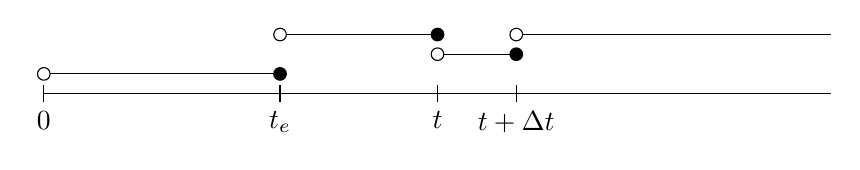
\begin{tikzpicture}
        \draw(0,0) -- (10,0);
        \foreach \x in {0,3,5,6}
            \draw (\x cm,3pt) -- (\x cm,-3pt);
        
        \draw (0,0) node[below=3pt] {$ 0 $};
        \draw (3,0) node[below=3pt] {$t_e$};
        \draw (5,0) node[below=3pt] {$t$};
        \draw (6,0) node[below=3pt] {$t+\Delta t$};
        
        \draw (0,.25) -- (3,.25);
        \draw (3,.75) -- (5, .75);
        \draw (6,.75) -- (10,.75);
        \draw (5,.5) -- (6,.5);
        
        \draw [fill=white] (0,.25) circle (0.08);
        \draw [fill=black] (3,.25) circle (0.08); 
        \draw [fill=white] (3,.75) circle (0.08);
        \draw [fill=black] (5,.75) circle (0.08);
        \draw [fill=white] (5,.5) circle (0.08);
        \draw [fill=black] (6,.5) circle (0.08);
        \draw [fill=white] (6,.75) circle (0.08);
    \end{tikzpicture}
    \caption{A partition of the timeline}
    \label{fig:partition}
\end{figure}
Thus $M(t_e)$ is the number of failures in $I_1$, $M(t+\Delta t)-M(t)$ is the number of failures in $I_2$ and $u-M(t+\Delta t) + M(t)-M(t_e)$ is the number of bugs in $I_3$. The probability of a failure occurring in each interval can be similarly found. Then
$$\mathbf{X}=(X_1,X_2,X_3)=\big(M(t_e), M(t+\Delta t)-M(t), u-M(t+\Delta t)+M(t)-M(t_e)\big)$$ 
with parameters $u$ and probability vector
$$(p_1, p_2, p_3)=\big(F(t_e), F(t+\Delta t)-F(t), 1-F(t+\Delta t)+F(t)-F(t_e)\big)$$ 
is a multinomial random variable. So
\begin{equation}\label{eq:prob-no-fail}
    \begin{aligned}
    \p(\text{no failure in } &(t, t+\Delta t] \; | \; M(t_e) = m_e) = \p(X_2 = 0 \;|\; X_1 = m_e)\\
    &= \frac{\p(X_1 = m_e, X_2=0, X_3=u-m_e)}{\p(X_1 =m_e)}\\
    &=\frac{{u\choose m_e,0, u-m_e}p_1^{m_e}p_2^0 p_3^{u-m_e}}{{u\choose m_e} p_1^{m_e}(1-p_1)^{u-m_e}}\\
    &=\left(\frac{p_3}{1-p_1}\right)^{u-m_e}\\
    &=\left(1 - \frac{F(t+\Delta t) - F(t)}{1 - F(t_e)}\right)^{u-m_e}.
\end{aligned}
\end{equation}
is the probability of the software running without failure in the near future. 

Let the conditional failure intensity at time $t\geq t_e$ be defined as
$$
\lambda(t\mid M(t_e)=m_e)=\lim_{\Delta t \to 0^+}\frac{1}{\Delta t}\p\big(\text{at least one failure in }(t,t+\Delta t]\mid M(t_e)=m_e\big).
$$
Recall that
\begin{align*}
    \p(\text{at least one failure in } &(t, t+\Delta t] \; | \; M(t_e) = m_e) \\&= 1 - \p(\text{no failure in } (t, t+\Delta t] \; | \; M(t_e) = m_e), 
\end{align*}
and so
\begin{align*}
    \lambda(t&\mid M(t_e)=m_e)\\
    &=\lim_{\Delta t\to 0^+}\frac{\p(M(t+\Delta t)-M(t) > 0)}{\Delta t}\\
    &=\lim_{\Delta t\to 0^+}\frac{1-\left(1 - \frac{F(t+\Delta t) - F(t)}{1 - F(t_e)}\right)^{u-m_e}}{\Delta t}&&(\text{By (\ref{eq:prob-no-fail})})\\
    &=\lim_{\Delta t\to 0^+}(u-m_e)\left(1 - \frac{F(t+\Delta t) - F(t)}{1 - F(t_e)}\right)^{u-m_e-1}\left(\frac{f(t+\Delta t)}{1-F(t_e)}\right)&&(\text{By l'Hopital})\\
    &=(u-m_e)\frac{f(t)}{1-F(t_e)}
\end{align*}

This quantity is useful since it allows one to find the expected number of failures in the near future given that $m_e$ failures occurred. Let $t=t_e$. Then the partition becomes $(0,t_e], (t_e, t_e+\Delta t], (t_e+\Delta t, \infty)$. Note that
\begin{align*}
    \p(X_2=k\mid X_1=m_e)&=\frac{\p(X_1=m_e, X_2=k, X_3=u-m_e-k)}{\p(X_1=m_e)}\\
    &=\frac{\frac{u!}{m_e!k!(u-m_e-k)!}p_1^{m_e}p_2^k p_3^{u-m_e-k}}{\frac{u!}{m_e!(u-m_e)!}p_1^{m_e}(1-p_1)^{u-m_e}}\\
    &={u-m_e\choose k}\left(\frac{p_2}{p_2+p_3}\right)^{u-m_e}\left(\frac{p_3}{p_2+p_3}\right)^{u-m_e-k}
\end{align*}
is binomially distributed with parameters $u-m_e$ and $\frac{p_2}{p_2+p_3}$. Therefore the conditional expectation is
\begin{equation}\label{eq:conditional_expectation}
        \begin{aligned}
        \Tilde{\mu}(t)&=\E(X_2\mid X_1=m_e)\\
        &=(u-m_e)\frac{p_2}{p_2+p_3}&&(\text{Expectation of binomial ditribution})\\
        &=(u-m_e)\frac{F(t_e+\Delta t)-F(t_e)}{1-F(t_e)}\\
        &=\int_0^{\Delta t}(u-m_e)\frac{f(t_e+t)}{1-F(t_e)}\,dt\\
        &=\int_0^{\Delta t}\lambda(t_e+t\mid X_1=m_e)\,dt.
\end{aligned}
\end{equation}

Suppose the management at MathWorks requires that the software will run for 4 CPU hours (14,400 CPU seconds) without failure with probability of 95\%. If, for example, at time $t_e$, $m_e=90$ out of $u=100$ bugs were found and fix, how reliable is the software?
To find the probability we need to decide on a distribution function. Since the bugs are independent and equally likely to cause a failure, the failures times are independent and occur a constant average rate. Thus letting $F(t)=1-e^{-\beta t}$ is the natural choice. Letting $\beta=10^{-6}$ and plugging all these values to Equation (\ref{eq:prob-no-fail}) we get
\begin{align*}
    \p(\text{no failure in } (t_e, t_e+\Delta t] \; | \; M(t_e) = m_e) &= \left(1 -\frac{F(t_e+\Delta t) - F(t_e)}{1 - F(t_e)}\right)^{u-m_e}\\&=e^{-0.144}\\&\approx0.866,
\end{align*}
and so more testing is needed. But how much? Let $\Tilde{t}$ be the additional testing time needed for the software to meet the requirements. We know that the probability of no failure in $(t, t+\Delta t]$ with $t=t_e+\Tilde{t}$ is given by 
$$
    \left(1-\frac{F(t_e+\Tilde{t}+\Delta t)-F(t_e+\Tilde{t})}{1-F(t_e)}\right)^{u-m_e}=\left(1-\frac{e^{-\beta(t_e+\Tilde{t})}-e^{-\beta(t_e+\Tilde{t}+\Delta t)}}{e^{-\beta t_e}}\right)^{u-m_e}.
$$
Setting the above equation to 0.95 and solving for $\Tilde{t}$ we obtain
\begin{equation}\label{eq:remaining-time}
    \Tilde{t}=-\frac{\log \frac{1-0.95^{\frac{1}{u-m_e}}}{1-e^{-\beta\Delta t}}}{\beta}.
\end{equation}
Hence the abovementioned example would require additional $\Tilde{t}=1.02763\times 10^6$ CPU seconds of testing or about 12 days for the software to meet the requirements.